% This file was created by tikzplotlib v0.9.1.
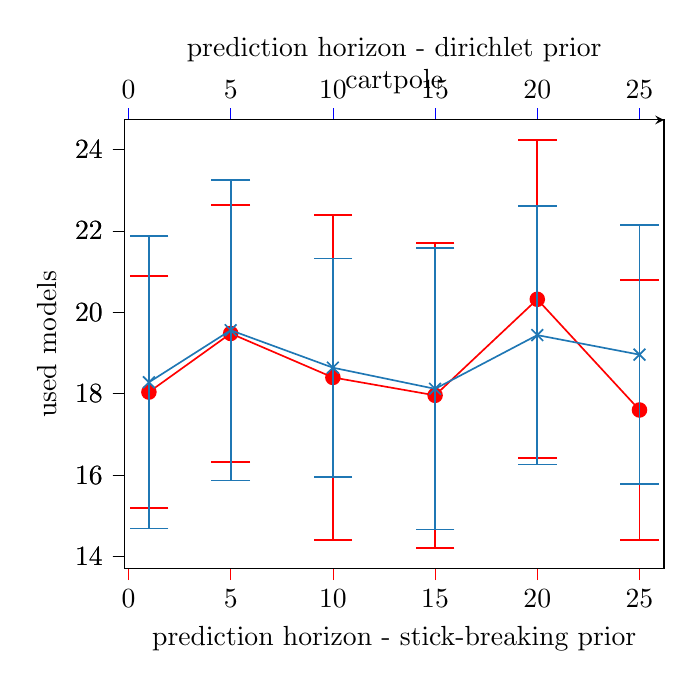
\begin{tikzpicture}

\definecolor{color0}{rgb}{0.12156862745098,0.466666666666667,0.705882352941177}

\begin{axis}[
tick align=outside,
tick pos=left,
title={cartpole},
x grid style={white!69.0196078431373!black},
xlabel={prediction horizon - stick-breaking prior},
xmin=-0.2, xmax=26.2,
xtick style={color=red},
y grid style={white!69.0196078431373!black},
ylabel={used models},
ymin=13.7125705569598, ymax=24.7267419513241,
ytick style={color=black}
]
\path [draw=red, semithick]
(axis cs:1,15.1907193890387)
--(axis cs:1,20.8892806109613);

\path [draw=red, semithick]
(axis cs:5,16.328873217403)
--(axis cs:5,22.631126782597);

\path [draw=red, semithick]
(axis cs:10,14.410012531348)
--(axis cs:10,22.389987468652);

\path [draw=red, semithick]
(axis cs:15,14.2132147112491)
--(axis cs:15,21.7067852887509);

\path [draw=red, semithick]
(axis cs:20,16.4139022029652)
--(axis cs:20,24.2260977970348);

\path [draw=red, semithick]
(axis cs:25,14.4)
--(axis cs:25,20.8);

\addplot [semithick, red, mark=-, mark size=7, mark options={solid}, only marks]
table {%
1 15.1907193890387
5 16.328873217403
10 14.410012531348
15 14.2132147112491
20 16.4139022029652
25 14.4
};
\addplot [semithick, red, mark=-, mark size=7, mark options={solid}, only marks]
table {%
1 20.8892806109613
5 22.631126782597
10 22.389987468652
15 21.7067852887509
20 24.2260977970348
25 20.8
};
\addplot [semithick, red, mark=*, mark size=2.5, mark options={solid}]
table {%
1 18.04
5 19.48
10 18.4
15 17.96
20 20.32
25 17.6
};
\end{axis}

\begin{axis}[
axis x line=top,
tick align=outside,
x grid style={white!69.0196078431373!black},
xlabel={prediction horizon - dirichlet prior},
xmin=-0.2, xmax=26.2,
xtick pos=right,
xtick style={color=blue},
y grid style={white!69.0196078431373!black},
ymin=13.7125705569598, ymax=24.7267419513241,
ytick pos=left,
ytick style={color=black}
]
\path [draw=color0, semithick]
(axis cs:1,14.6853372898142)
--(axis cs:1,21.8746627101858);

\path [draw=color0, semithick]
(axis cs:5,15.8713145973125)
--(axis cs:5,23.2486854026875);

\path [draw=color0, semithick]
(axis cs:10,15.9585078780649)
--(axis cs:10,21.3214921219351);

\path [draw=color0, semithick]
(axis cs:15,14.6637592676435)
--(axis cs:15,21.5762407323565);

\path [draw=color0, semithick]
(axis cs:20,16.2640906813953)
--(axis cs:20,22.6159093186047);

\path [draw=color0, semithick]
(axis cs:25,15.7790567436686)
--(axis cs:25,22.1409432563314);

\addplot [semithick, color0, mark=-, mark size=7, mark options={solid}, only marks]
table {%
1 14.6853372898142
5 15.8713145973125
10 15.9585078780649
15 14.6637592676435
20 16.2640906813953
25 15.7790567436686
};
\addplot [semithick, color0, mark=-, mark size=7, mark options={solid}, only marks]
table {%
1 21.8746627101858
5 23.2486854026875
10 21.3214921219351
15 21.5762407323565
20 22.6159093186047
25 22.1409432563314
};
\addplot [semithick, color0, mark=x, mark size=3, mark options={solid}]
table {%
1 18.28
5 19.56
10 18.64
15 18.12
20 19.44
25 18.96
};
\end{axis}

\end{tikzpicture}
